%!TEX options = --shell-escape

\documentclass[bachelor]{thesis-uestc}

\title{基于tus协议的断点续传客户端软件}
\author{唐治中}
\advisor{丘志杰\chinesespace 高级工程师}
\school{计算机科学与工程学院}
\major{计算机科学与技术}
\studentid{2014060107011}

\usepackage{tabu}
\usepackage{listings}
\lstset{
 %basicstyle=\fontspec{SimHei},
 basicstyle=\footnotesize \ttfamily,
 breaklines=true,                                  %这条命令可以让LaTeX自动将长的代码行换行排版
 extendedchars=true,                               %解决代码跨页时,章节标题,页眉等汉字不显示的问题
 columns=fixed,       
 numbers=left,                                     % 在左侧显示行号
 numberstyle=\tiny\color{gray},                    % 设定行号格式
 frame=shadowbox,                                  % 显示背景边框
 backgroundcolor=\color[RGB]{245,245,244},         % 设定背景颜色
 keywordstyle=\color[RGB]{40,40,255},              % 设定关键字颜色
 numberstyle=\footnotesize\color{darkgray},           
 commentstyle=\it\color[RGB]{0,96,96},             % 设置代码注释的格式
 stringstyle=\rmfamily\slshape\color[RGB]{128,0,0},% 设置字符串格式
 showstringspaces=false,                           % 不显示字符串中的空格
 language=java,                                    % 设置语言
}
%\begin{lstlisting}[title=Myfile, frame=shadowbox]
%代码
%\end{lstlisting}

\setcounter{secnumdepth}{4} % 编号的深度,4 表示到 paragraph 一级,默认为 2
\setcounter{tocdepth}{4} % 目录中的深度

\begin{document}

\makecover

\begin{chineseabstract}
为了适应当下日益增长的用户对文件传输的多样化需求,断点续传功能作为一项保证文件传输质量的技术得到了广泛的应用。本文以tus传输协议为研究课题,实现了基于tus协议的断点续传客户端软件的开发,重点实现了文件传输过程中按块传输的方法,通过配置文件记录传输位置以便继续传输,使用多线程传输文件等。本软件使用JAVA语言实现,实现内容分为四部分,分别是协议基本内容,具体功能和模块,软件的编程实现详述,以及测试软件功能和完善。
\par 其中,tus协议的基本内容是对tus协议的解读与理解,包含了请求格式的详细介绍。软件的具体功能和模块设计部分介绍了本软件的需求分析,类的详细划分,以及程序的主要流程和对应类间的调用关系。软件的编程实现内容中,主要展示了软件核心类的代码详述,对应各个功能模块的代码实现。在软件测试部分中,通过编写测试用例的方式测试了主要函数的功能正确性,以及对软件的稳定性的简单测试。



\chinesekeyword{tus协议,断点续传,JAVA,配置文件,多线程}
\end{chineseabstract}

\begin{englishabstract}
In order to adapt to the ever-increasing user demand for the diversification of file transfer, the breakpoint resume function has been widely used as a technology for guaranteeing the file transfer quality. This article takes the tus transmission protocol as the research topic, realizes the development of the client software of the broken point resuming client based on the tus protocol, focuses on the method of block transmission in the file transmission process, records the transmission position through the configuration file to continue transmission, and uses multithreading transfer files and so on. The software is implemented in JAVA language. The implementation is divided into four parts, which are the basic contents of the agreement, specific functions and modules, detailed programming of the software, and testing software functions and improvements.
\par Among them, the basic content of the tus protocol is the interpretation and understanding of the tus protocol, including a detailed description of the request format. The software's specific function and module design section introduces the software's requirement analysis, the detailed division of the class, and the main flow of the program and the corresponding relationship between the classes. In the programming and implementation content of the software, the code of the core class of the software is shown in detail, corresponding to the code implementation of each functional module. In the software testing part, the function correctness of the main function is tested by writing test cases, and a simple test of the stability of the software is performed.

\englishkeyword{file transfer, breakpoint resume, tus transmission protocol, transmission by block, multi-threaded transfer, programming environment}
\end{englishabstract}

\thesistableofcontents

\thesischapterexordium

\section{研究工作的背景}
HTTP超文本传输协议,是一种用于分布式、协作式和超媒体信息系统的应用层协议。HTTP是万维网的数据通信的基础。设计HTTP最初的目的是为了提供一种发布和接收HTML页面的方法。通过HTTP或者HTTPS协议请求的资源由统一资源标识符来标识。而如今的http协议的发展前景是,将web服务器内置到嵌入式工控节点,由网络服务器提供交互式Internet服务,例如提供符合http协议的用户远程监控界面和信息交互服务。在web嵌入式远程监控系统中\citing{qianrushi},将被监控的各底层状态定义成HTML语言许可的网络变量,然后利用这些变量生成网页,由网络服务器提供给远程用户,远程用户使用网络浏览器,下载服务器上的页面,以观察设备的实时运行情况,远程修改这些变量,完成对现场设备的监控。而对于这种http协议的嵌入式应用同样也需要断点续传的支持,使这些设备监控功能更加完善。
\par 通过 HTTP,可以非常方便的实现断点续传。断点续传主要依赖于 HTTP 头部定义的 Range 来完成。具体 Range 的说明参见 RFC2616中 14.35.2 节,在请求某范围内的资源时,可以更有效地对大资源发出请求或从传输错误中恢复下载。有了 Range,应用可以通过 HTTP 请求曾经获取失败的资源的某一个返回或者是部分,来恢复下载该资源。当然并不是所有的服务器都支持 Range,但大多数服务器是可以的。Range 是以字节计算的,请求的时候不必给出结尾字节数,因为请求方并不一定知道资源的大小。


\section{断点续传的现状与意义}
断点续传:指的是在上传/下载时,将任务(一个文件或压缩包)人为的划分为几个部分,每一个部分采用一个线程进行上传/下载,如果碰到网络故障,可以从已经上传/下载的部分开始继续上传/下载未完成的部分,而没有必要从头开始上传/下载。可以节省时间,提高速度。
\par 有时用户上传/下载文件需要历时数小时,万一线路中断,不具备断点续传的 HTTP/FTP 服务器或下载软件就只能从头重传,比较好的 HTTP/FTP 服务器或下载软件具有断点续传能力,允许用户从上传/下载断线的地方继续传送,这样大大减少了用户的烦恼。
\par 本课题的tus断点续传功能的实现对于现如今的网络时代有着非常重要的意义,只要是通过网络进行交流的终端间,和使用http协议进行传输的终端间,就存在着因特殊情况而出现的传输中断,而断点续传功能的应用就可以有效的避免这些因为硬件故障或人为操作失误所带来的损失,从而提高用户间的交流效率,使网络空间更加高效便利可靠。

\section{实现本软件的主要工作内容}
本软件利用JAVA语言,以及tus官方提供的tus服务器端软件,实现了客户端的基本功能,主要工作内容如下:
\par 本软件基本实现了tus协议规定的文件传输要求,例如按照tus协议内容规范请求报文以及返回信息格式,用JAVA实现了断点续传的基本功能,核心类封装了传输所需的信息,提供了参数及接口,便于在此基本功能上进行拓展。突出点在于使用了多线程技术管理传输过程。

\section{本论文的结构安排}
本文的章节结构安排如下:
\par 第一章绪论主要介绍了本课题的工作背景,断点续传功能的现状及意义,本设计的主要工作等。第二章介绍了tus的协议基础,第三章详细描述了软件的功能及模块设计,第四章着重展示通过具体的编程语言来实现软件功能和模块的过程。第五章展示了软件的测试与成果展示。

\chapter{tus协议基础}
tus协议提供了一种通过HTTP / 1.1(RFC 7230)\citing{rfc7230} 和HTTP / 2(RFC 7540)\citing{rfc7540} 进行可恢复文件上传的机制。

\section{tus核心协议}
核心协议介绍了如何恢复中断上传。 它假定您已经有了上传的URL,通常是通过创建扩展名创建的。
所有客户端和服务器必须实施核心协议。
本规范没有描述URL的结构,因为这是由具体实现决定的。 本文档中显示的所有URL仅用于举例目的。
另外,服务器决定执行认证和授权\citing{tusio}。

\subsection{tus请求}
\subsubsection{HEAD}
即使偏移量为0,或者上传已被视为已完成,服务器必须始终在HEAD请求的响应中包含上载偏移头。 如果上传的大小已知,则服务器必须在响应中包含Upload-Length头。 如果没有找到该资源,服务器应该返回404 Not Found,410 Gone或403 Forbidden状态,而没有Upload-Offset头。
\par 服务器必须通过向响应添加Cache-Control:no-store头来防止客户端和/或代理缓存响应。
\par HEAD请求用于确定应继续上传的偏移量。
下面的示例显示了在传输70个字节后中断的100字节上传的继续。
\begin{lstlisting}[title=Request]
HEAD /files/24e533e02ec3bc40c387f1a0e460e216 HTTP/1.1
Host: tus.example.org
Tus-Resumable: 1.0.0
\end{lstlisting}

\begin{lstlisting}[title=Response]
HTTP/1.1 200 OK
Upload-Offset: 70
Tus-Resumable: 1.0.0
\end{lstlisting}

\subsubsection{PATCH}
服务器应该接受针对任何上传URL的PATCH请求,并在由上传偏移头指定的给定偏移量处应用消息中包含的字节。所有的PATCH请求必须使用Content-Type:application / offset + octet-stream。

上传偏移报头的值必须等于资源的当前偏移量。为了实现并行上传,可以使用级联扩展。如果偏移量不匹配,服务器必须响应409冲突状态而不修改上传资源。

客户端应该在一个PATCH请求中发送所有剩余的上传字节,但也可以在需要的情况下连续使用多个小的请求。这种情况的一个例子是当使用Checksum扩展时。

服务器务必确认成功的PATCH请求204无内容状态。它必须包含包含新偏移量的Upload-Offset头。新的偏移量必须是PATCH请求之前的偏移量与当前PATCH请求期间接收和处理或存储的字节数之和。

客户端和服务器都应该尝试检测并处理可预测的网络错误。他们可以通过检查读/写套接字错误以及设置读/写超时来做到这一点。超时应该通过关闭底层连接来处理。

服务器应该总是尝试存储尽可能多的接收数据。
\par 鉴于偏移量,客户端使用PATCH方法恢复上传:
\begin{lstlisting}[title=Request]
PATCH /files/24e533e02ec3bc40c387f1a0e460e216 HTTP/1.1
Host: tus.example.org
Content-Type: application/offset+octet-stream
Content-Length: 30
Upload-Offset: 70
Tus-Resumable: 1.0.0
\end{lstlisting}

\begin{lstlisting}[title=Response]
HTTP/1.1 204 No Content
Tus-Resumable: 1.0.0
Upload-Offset: 100
\end{lstlisting}

\subsubsection{OPTION}
OPTIONS请求可以用来收集关于服务器当前配置的信息。 由204无内容或200 OK状态指示的成功响应必须包含Tus-Version标头。 它可能包含Tus-Extension和Tus-Max-Size标题。

客户端不应该在请求中包含Tus-Resumable头,服务器必须忽略头。

本示例阐明了对OPTIONS请求的响应。 在请求和响应中使用的版本是1.0.0,而服务器也能够处理0.2.2和0.2.1。 上传总数最多为1GB,允许创建和过期的扩展。
\begin{lstlisting}[title=Request]
OPTIONS /files HTTP/1.1
Host: tus.example.org
\end{lstlisting}

\begin{lstlisting}[title=Response]
HTTP/1.1 204 No Content
Tus-Resumable: 1.0.0
Tus-Version: 1.0.0,0.2.2,0.2.1
Tus-Max-Size: 1073741824
Tus-Extension: creation,expiration
\end{lstlisting}

\section{tus协议的头部信息}
头部信息Headers中包含了在发送请求和返回相应信息中的关键字。

1.Upload-Offset:Upload-Offset请求和响应头指示资源内的字节偏移。 该值必须是一个非负整数。

2.Upload-Length:上传长度请求和响应标头以字节表示整个上传的大小。 该值必须是一个非负整数。

3.Tus-Version:Tus-Version响应头必须是服务器支持的协议版本的逗号分隔列表。 该列表务必按照服务器的首选项排序,其中第一个是最优选的。

4.Tus-Resumable:除OPTIONS请求外,Tus可恢复头部必须包含在每个请求和响应中。 该值必须是客户端或服务器使用的协议版本。
\par 如果客户端指定的版本不被服务器支持,它必须响应412 Precondition Failed状态,并且必须在响应中包含Tus-Version标头。 另外,服务器不能处理请求。

5.Tus-Extension:Tus-Extension响应头必须是服务器支持的扩展名的逗号分隔列表。 如果不支持扩展,则必须省略Tus-Extension头。

6.Tus-Max-Size:Tus-Max-Size响应头必须是一个非负整数,指示整个上传允许的最大字节大小。 如果存在已知的硬限制,服务器应该设置该标头。

7.X-HTTP-Method-Override:如果头部出现,X-HTTP-Method-Override请求头必须是一个必须被服务器解释为请求方法的字符串。 请求的实际方法必须被忽略。 如果客户端环境不支持PATCH或DELETE方法,客户端应该使用这个头文件。

\section{tus协议扩展}
鼓励客户和服务器尽可能多地实现扩展。 功能检测应该通过客户端发送OPTIONS请求和服务器响应Tus-Extension头来实现。

\subsection{新建上传}
客户端和服务器应该实现上传创建扩展。 如果服务器支持这个扩展,它必须添加创建到Tus-Extension头。
\subsubsection{举例}
一个空的POST请求用于创建一个新的上传资源。 上传长度标题以字节表示整个上传的大小。
\begin{lstlisting}[title=Request]
POST /files HTTP/1.1
Host: tus.example.org
Content-Length: 0
Upload-Length: 100
Tus-Resumable: 1.0.0
Upload-Metadata: filename d29ybGRfZG9taW5hdGlvbl9wbGFuLnBkZg==
\end{lstlisting}
\begin{lstlisting}[title=Response, language=]
HTTP/1.1 201 Created
Location: https://tus.example.org/files/24e533e02ec3bc40c387f1a0e460e216
Tus-Resumable: 1.0.0
\end{lstlisting}
新资源的隐含偏移量为0,允许客户端使用核心协议来执行实际上传。
\subsubsection{头部信息}
1.Upload-Defer-Length:Upload-Defer-Length请求和响应标头指示上传的大小当前不知道,并且稍后将被传输。 它的值必须是1.如果上传的长度没有延迟,这个头部必须省略。

2.Upload-Metadata:上传元数据请求和响应头必须由一个或多个以逗号分隔的键值对组成。 密钥和值必须用空格分隔。 密钥不能包含空格和逗号,也不能为空。 该键应该是ASCII编码的,并且该值必须是Base64编码的。 所有密钥必须是唯一的。
\subsubsection{要求}
客户端必须发送一个针对已知上传创建URL的POST请求来请求一个新的上传资源。该请求必须包含以下标题之一:
\par a)上传长度以字节表示整个上传的大小。
\par b)上传 - 推迟 - 长度:如果上传大小当时未知,则为1。一旦知道客户端必须在下一个PATCH请求中设置上传长度标题。一旦设定的长度不能改变。只要上传长度未知,服务器必须在对HEAD请求的所有响应中设置上传延迟长度:1。
\par 如果服务器支持推迟长度,它必须添加创建 - 延迟长度到Tus-Extension报头。
\par 客户端可以提供上传 - 元数据头部以向上传创建请求添加额外的元数据。服务器可以决定忽略或使用这些信息来进一步处理请求或拒绝它。如果上传包含额外的元数据,对HEAD请求的响应必须包含上传 - 元数据头及其在创建期间由客户指定的值。
\par 如果上传的长度超过了最大值(可以使用Tus-Max-Size头部指定),那么服务器必须响应413请求实体太大的状态。
\par 服务器必须通过201 Created状态确认成功上传创建。服务器必须将Location标头设置为所创建资源的URL。这个网址可能是绝对的或相对的。
\par 客户端必须使用核心协议执行实际上传。

\subsection{过期处理}
服务器可以在它们到期后删除未完成的上传。 为了向客户端表明这种行为,服务器必须将过期添加到Tus-Extension报头。
\subsubsection{举例}
在Upload-Expires中指定的时间之前,未完成的上传可用。 此日期之后,上传无法恢复。
\begin{lstlisting}[title=Request]
PATCH /files/24e533e02ec3bc40c387f1a0e460e216 HTTP/1.1
Host: tus.example.org
Content-Type: application/offset+octet-stream
Content-Length: 30
Upload-Offset: 70
Tus-Resumable: 1.0.0
\end{lstlisting}
\begin{lstlisting}[title=Response, language=]
HTTP/1.1 204 No Content
Upload-Expires: Wed, 25 Jun 2014 16:00:00 GMT
Tus-Resumable: 1.0.0
Upload-Offset: 100
\end{lstlisting}
\subsubsection{头部信息}
1.Upload-Expires:Upload-Expires响应标题指示未完成上载过期的时间。 服务器可能希望在一段时间后删除不完整的上传,以防止被放弃的上传占用额外的存储空间。 客户端应该使用这个头部来确定在尝试恢复上传之前上传是否仍然有效。
\par 如果上传过期,该头部必须包含在每个PATCH响应中。 如果在创建时已知过期,则Upload-Expires标头必须包含在对初始POST请求的响应中。 它的值可能会随着时间而改变。
\par 如果客户端尝试恢复已被服务器删除的上载,则服务器应该以404 Not Found或410 Gone状态进行响应。 如果服务器正在跟踪过期的上传,则应使用后者。 在这两种情况下,客户端都应该开始新的上传。
\par Upload-Expires头的值必须采用RFC 7231 datetime格式。

\subsection{校验处理}
客户端和服务器可以实现并使用此扩展来验证每个PATCH请求的数据完整性。如果支持,服务器必须将校验和添加到Tus-Extension头。
\par 客户端可以在PATCH请求中包含Upload-Checksum标头。一旦收到完整的请求,服务器必须使用指定的算法验证上传的块对照提供的校验和。取决于结果,服务器可以用以下状态码之一响应:1)如果服务器不支持校验和算法,则为400错误请求; 2)460校验和不匹配,如果校验和不匹配;或者3)204如果校验和匹配和数据处理成功。在前两种情况下,必须丢弃上传的块,并且不得更新上传及其偏移量。
\par 服务器必须至少支持由sha1标识的SHA1校验和算法。校验和算法的名称只能由ASCII字符组成,修改后不包括大写字符。
\par Tus-Checksum-Algorithm头必须包含在OPTIONS请求的响应中。
\par 如果散列不能在上传开始时计算,则可以将其作为预告片加入。如果服务器可以处理预告片,则必须通过向Tus-Extension头添加校验和预告片来宣布此行为。预告片,也称为尾部标题,是在请求正文已经传输之后发送的标题。遵循RFC 7230,它们必须使用尾部标头进行宣布,并且只允许在分块传输中使用。
\subsubsection{头部信息}
1.Tus-Checksum-Algorithm:Tus-Checksum-Algorithm响应头必须是服务器支持的校验和算法的逗号分隔列表。

2.Upload-Checksum:Upload-Checksum请求标头包含有关当前主体有效负载校验和的信息。 头部必须由用空格分隔的校验和算法的名称和Base64编码的校验和组成。
\subsubsection{举例}
\begin{lstlisting}[title=Request]
OPTIONS /files HTTP/1.1
Host: tus.example.org
Tus-Resumable: 1.0.0
\end{lstlisting}
\begin{lstlisting}[title=Response]
HTTP/1.1 204 No Content
Tus-Resumable: 1.0.0
Tus-Version: 1.0.0
Tus-Extension: checksum
Tus-Checksum-Algorithm: md5,sha1,crc32
\end{lstlisting}
\begin{lstlisting}[title=Request]
PATCH /files/17f44dbe1c4bace0e18ab850cf2b3a83 HTTP/1.1
Content-Length: 11
Upload-Offset: 0
Tus-Resumable: 1.0.0
Upload-Checksum: sha1 Kq5sNclPz7QV2+lfQIuc6R7oRu0=

hello world
\end{lstlisting}
\begin{lstlisting}[title=Response]
HTTP/1.1 204 No Content
Tus-Resumable: 1.0.0
Upload-Offset: 11
\end{lstlisting}

\subsection{终止处理}
该扩展为客户端定义了一种终止已完成和未完成的上传的方式,允许服务器释放已用资源。
\par 如果服务器支持该扩展,则必须通过向Tus-Extension头添加终止来宣布。
\subsubsection{需求}
当接收到一个现有上传的DELETE请求时,服务器应该释放相关的资源,并且必须响应204无内容状态,确认上传已经终止。 对于将来对这个URL的所有请求,服务器应该用404 Not Found或410 Gone状态进行响应。
\subsubsection{举例}
\begin{lstlisting}[title=Request]
DELETE /files/24e533e02ec3bc40c387f1a0e460e216 HTTP/1.1
Host: tus.example.org
Content-Length: 0
Tus-Resumable: 1.0.0
\end{lstlisting}
\begin{lstlisting}[title=Response]
HTTP/1.1 204 No Content
Tus-Resumable: 1.0.0
\end{lstlisting}

\subsection{级联处理}
该扩展可用于将多个上传连接为一个上传,使客户端可以执行并行上传并上传不连续的块。如果服务器支持这个扩展,它必须添加连接到Tus-Extension头。
\par 部分上传代表一个文件块。它通过包含Upload-Concat:部分头部来创建,同时使用创建扩展创建新的上传。多个部分上传按指定顺序连接成最终上传。服务器不应该处理这些部分上传,直到它们连接在一起形成最终上传。最终上传的长度必须是所有部分上传长度的总和。
\par 为了创建新的最终上传,客户端必须将Upload-Concat头添加到上传创建请求中。该值必须是最后的,后跟需要连接的部分上传URL的分号和空格分隔的列表。部分上传必须按照列表中指定的顺序进行连接。这个连接请求应该在所有相应的部分上传完成之后发生。客户端不得在最终的上传创建中包含上传长度标题。
\par 当部分上传仍在进行中时,客户端可以发送连接请求。这个特性必须由服务器通过向Tus扩展头添加未完成的连接来明确地宣布。
\par 当创建新的最终上传时,部分上传的元数据不会被传输到新的最终上传。所有元数据都应该使用Upload-Metadata头部包含在串联请求中。
\par 服务器可以在连接后删除部分上传。然而,它们可能会被多次使用以形成最终资源。
\par 服务器必须以403禁止状态响应最终上传URL的PATCH请求,并且不得修改最终上传或其部分上传。
\par 对最终上载的HEAD请求的响应不应包含Upload-Offset标头,除非级联已成功完成。成功连接后,必须设置Upload-Offset和Upload-Length,它们的值必须相等。没有为最终上载定义连接前的Upload-Offset头的值。
\par 对HEAD请求进行部分上传的响应必须包含上传偏移头。
\par 如果可以在请求时计算最终资源的长度,则必须包含上传长度标题。针对部分或最终上传的HEAD请求的响应必须包含上传创建请求中收到的Upload-Concat标头及其值。
\subsubsection{头部信息}
1.Upload-Concat:Upload-Concat请求和响应头部必须在部分和最终上传创建请求中设置。 它指示上传是部分还是最终上传。 如果上传是部分内容,则标头值必须是部分的。 在最终上传的情况下,它的值必须是最后的,后跟一个分号和空格分隔的部分上传URL列表,它们将被连接起来。 部分上传的URL可能是绝对的或相对的,并且不能包含RFC 3986中定义的空格。
\subsubsection{举例}
在下面的例子中,为了便于阅读,省略了Host和Tus-Resumable头文件,尽管它们是规范要求的。 在开始时创建两个部分上传:
\begin{lstlisting}[title=第一部分, language=]
POST /files HTTP/1.1
Upload-Concat: partial
Upload-Length: 5

HTTP/1.1 201 Created
Location: https://tus.example.org/files/a
\end{lstlisting}
\begin{lstlisting}[title=第二部分, language=]
POST /files HTTP/1.1
Upload-Concat: partial
Upload-Length: 6

HTTP/1.1 201 Created
Location: https://tus.example.org/files/b
\end{lstlisting}
现在可以使用PATCH请求将数据上传到两个部分资源:
\begin{lstlisting}[title=第一部分]
PATCH /files/a HTTP/1.1
Upload-Offset: 0
Content-Length: 5

hello

HTTP/1.1 204 No Content
\end{lstlisting}
\begin{lstlisting}[title=第二部分]
PATCH /files/b HTTP/1.1
Upload-Offset: 0
Content-Length: 6

 world

HTTP/1.1 204 No Content
\end{lstlisting}
在第一个请求中,字符串hello已上传,而第二个文件现在包含带有前导空格的“world”。
\par 下一步是创建包含两个较早生成的部分上传的最终上传。 在接下来的请求中,没有呈现上传长度标题。
\begin{lstlisting}[title=Request and Response, language=]
POST /files HTTP/1.1
Upload-Concat: final;/files/a /files/b

HTTP/1.1 201 Created
Location: https://tus.example.org/files/ab
\end{lstlisting}
最终资源的长度现在是11个字节,由字符串hello world组成。
\begin{lstlisting}[title=Request and Response, language=]
HEAD /files/ab HTTP/1.1

HTTP/1.1 200 OK
Upload-Length: 11
Upload-Concat: final;/files/a /files/b
\end{lstlisting}

\section{关于base64}
Base64是一种基于64个可打印字符来表示二进制数据的表示方法。由于$2^{6}$=64,所以每6个比特为一个单元,对应某个可打印字符。3个字节有24个比特,对应于4个Base64单元,即3个字节可由4个可打印字符来表示。它可用来作为电子邮件的传输编码。在Base64中的可打印字符包括字母A-Z、a-z、数字0-9,这样共有62个字符,此外两个可打印符号在不同的系统中而不同。一些如uuencode的其他编码方法,和之后BinHex的版本使用不同的64字符集来代表6个二进制数字,但是不被称为Base64\citing{base64}。



\begin{figure}[h]
\subfigure{
\label{man}
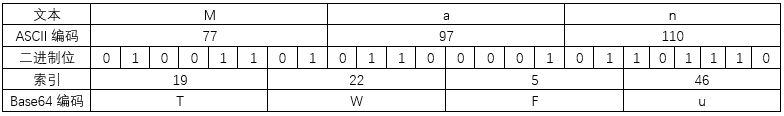
\includegraphics[width=15cm]{man.png}}
\caption{编码“Man”}
\end{figure}

如果要编码的字节数不能被3整除,最后会多出1个或2个字节,那么可以使用下面的方法进行处理:先使用0字节值在末尾补足,使其能够被3整除,然后再进行Base64的编码。在编码后的Base64文本后加上一个或两个=号,代表补足的字节数。也就是说,当最后剩余两个八位字节(2个byte)时,最后一个6位的Base64字节块有四位是0值,最后附加上两个等号;如果最后剩余一个八位字节(1个byte)时,最后一个6位的base字节块有两位是0值,最后附加一个等号。

\begin{figure}[h]
\subfigure{
\label{special}
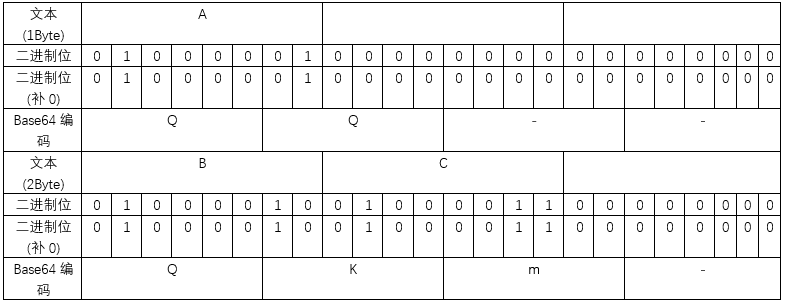
\includegraphics[width=15cm]{special.png}}
\caption{特殊处理}
\end{figure}

\begin{figure}[h]
\subfigure{
\label{base64}
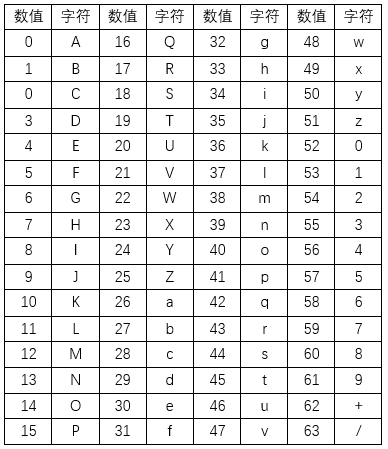
\includegraphics[width=6.77cm]{base64.png}}
\caption{Base64索引表}
\end{figure}

\section{JAVA语言的环境配置}
Java是一种广泛使用的电脑程式设计语言,拥有跨平台、物件导向、泛型程式设计的特性,广泛应用于企业级Web应用开发和移动应用开发。
\par Java编程语言的风格十分接近C++语言。继承了C++语言面向对象技术的核心,Java舍弃了C++语言中容易引起错误的指针,改以引用取代,同时移除了C++中的运算符重载和多重继承特性,改用接口取代,增加垃圾回收器功能。在Java SE 1.5版本中引入了泛型编程、类型安全的枚举、不定长参数和自动装/拆箱特性。昇阳电脑对Java语言的解释是:“Java编程语言是个简单、面向对象、分布式、解释性、健壮、安全与系统无关、可移植、高性能、多线程和动态的语言”\citing{java}

\subsection{JAVA工具包JDK}
Java Development Kit(JDK)是昇阳电脑针对Java开发人员发布的免费软件开发工具包(SDK,Software development kit)。自从Java推出以来,JDK已经成为使用最广泛的Java SDK。由于JDK的一部分特性采用商业许可证,而非开源\citing{jdk}。

\subsection{JAVA运行环境JRE}
Java执行环境(Java Runtime Environment,简称JRE)是一个软体,由昇阳电脑所研发,JRE可以让电脑系统执行Java应用程式(Java Application)。
\par JRE的内部有一个Java虚拟机器(Java Virtual Machine,JVM)以及一些标准的类别函数库(Class Library)\citing{jre}。

\subsection{JDK和JRE的安装}
首先下载\citing{jdkjredownload}安装\citing{jdkjreinstall}JDK和JRE的安装包。
\subsubsection{关于PC配置要求}
对于64位Windows平台,JDK和JRE具有最低的处理器,磁盘空间和内存要求。
\par 在64位Windows平台上安装JDK或JRE之前,必须验证它是否满足以下最低处理器,磁盘空间和内存要求。
\begin{figure}[h]
\subfigure{
\label{jdk}
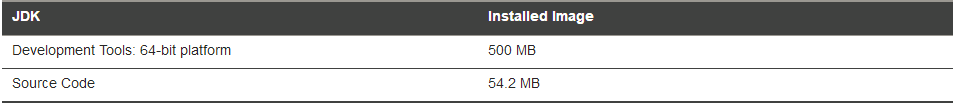
\includegraphics[width=12cm]{jdk.png}}
\caption{安装jdk的硬盘要求}
\end{figure}

\begin{figure}[h]
\subfigure{
\label{jre}
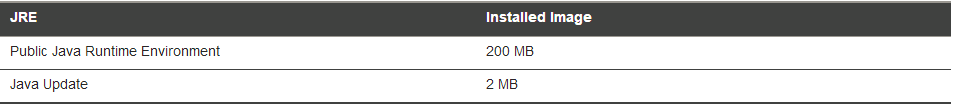
\includegraphics[width=12cm]{jre.png}}
\caption{安装jre的硬盘要求}
\end{figure}

\subsection{环境变量的配置}
添加JAVAHOME变量:
\begin{figure}[h]
\subfigure{
\label{javahome}
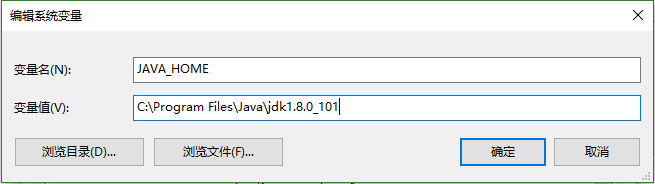
\includegraphics[width=12cm]{javahome.png}}
\caption{JAVAHOME变量的添加}
\end{figure}
\par 添加Path变量(如图3-4所示):
\begin{figure}[h]
\subfigure{
\label{path}
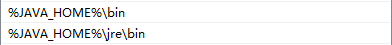
\includegraphics[width=12cm]{path.png}}
\caption{Path变量的添加}
\end{figure}
\par 在添加好环境变量后,可通过Windows的DOS窗口或者PowerShell使用java命令(如图3-5所示):
\begin{figure}[h]
\subfigure{
\label{powershell}
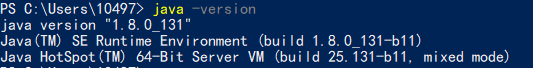
\includegraphics[width=12cm]{powershell.png}}
\caption{在Windows的PowerShell中查看java命令}
\end{figure}

\section{本章小结}
本章首先从tus协议本身开始,介绍了本断点续传软件遵循的协议理论基础,为软件的功能模块设计以及代码实现做好铺垫。

\chapter{软件的设计}


\section{需求分析与实现原理}
软件设计是程序员按照特定顺序撰写计算机数据和指令的集合。“软件设计”可以是撰写最基础的二进制0和1比特;也可以是创建在比特之上的各类软件语言、算法、架构、程序、图像化代码来进行\citing{xuqiu}。
\subsection{软件的需求分析}
本软件的结构原理图如图3-1:
\begin{figure}[h]
\subfigure{
\label{structure}
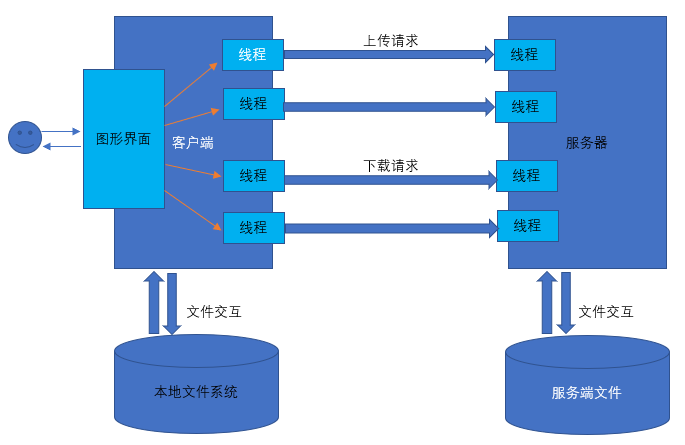
\includegraphics[width=13cm]{structure.png}}
\caption{文件传输软件结构图}
\end{figure}
如结构图所示,本客户端软件主要与服务器进行文件的交互,交互过程遵循tus协议,其中主要需求为:
\par 1.需要图形界面,与用户进行交互。
\par 2.需要管理并使用多线程与服务器发送请求和接受回复。
\par 3.需要与本地文件系统交互,完成文件的上传和下载,并包含与配置文件相关的操作。
\par 4.图3-1展示出的仅为普通文件传输的结构,要实现断点续传的功能,必须设计出循环按数据块传输文件的操作。
\par 补充说明:由于在这次毕业设计测试中,服务端选择的是官方提供的tusd软件,而tusd中已经包含了多线程的处理、遵循tus协议的请求与回复处理以及对于相同文件同时请求的锁处理,所以在客户端的编写中就没有进行文件的锁处理,只主要负责了相应的请求,文件的操作,配置文件的设计以及块传输的编写。
\par 关于按块传输:按块传输是断点续传功能的核心,将整个文件划分成固定大小的数据块,可将文件的传输作为一个循环,每次传输固定大小的数据块内容,这样才能在每次循环中记录下offset的值,以便在继续传输的时候使用offset作为传输的起点。
\par 普通的文件传输如下图3-2所示,inputstream的输入流是连续的概念,于是当中断发生时无法高效的记录此刻文件的传输位置即offset的值,这样当下次向继续传输时便无从下手。
\begin{figure}[h]
\subfigure{
\label{normal}
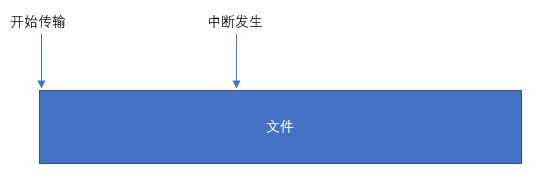
\includegraphics[width=13cm]{normal.png}}
\caption{普通的文件传输}
\end{figure}
\par 于是提供了如图3-3所示的分块传输的设计:将文件分成固定大小每块相等的数据块,并循环按块传输。这样的好处在于没传输一个数据块的数据之后就可以更新并记录文件传输位置即offset的值,当中断发生时,如3-3所示的情况,中断在数据块3传输过程中发生,这时offset记录的值为前一块数据块2传输完成后记录的值。此时虽然发生了中断,但程序成功记录了文件传输的offset值。
\par 因此,在下次需要继续传输的时候就可以通过offset值使传输起点从块2之后,块3之前的位置开始,完成断点续传的任务。
\par 而且,值得注意的是,为了保证断点续传软件的功能完整性,应该考虑到一些特殊情况下的offset记录设计。比如设置单独的传输暂停按钮和恢复传输按钮,使软件的功能更加完善。
\par 此外,tusd官方服务器提供了文件上传时服务端文件offset的记录过程,断点续传客户端只需在文件下载过程中提供文件传输位置offset的记录过程。
\begin{figure}[h]
\subfigure{
\label{chunk}
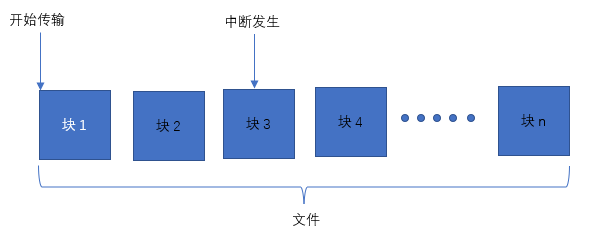
\includegraphics[width=14cm]{chunk.png}}
\caption{分块的循环文件传输}
\end{figure}



\section{软件的模块设计}
模块化编程(modular programming)是一种软件设计技术,它将软件分解为若干独立 的、可替换的、具有预定功能的模块,每个模块实现一个功能,各模块通过接口(输入输出 部分)组合在一起,形成最终程序。
对于简单问题,可以直接构建单一模块的程序。而对于复杂问题,则可以先创建若干个较小的模块,然后将它们组装、链接在一起,从而构成复杂的软件系统。模块化编程具有以 下优点:
\par 易设计:较大的复杂问题分解为若干较小的简单问题,使我们可以从抽象的模块功 能角度而非具体的实现角度去理解软件系统,从而整个系统的结构非常清晰、容易 理解,设计人员在设计之初可以更加关注系统的顶层逻辑而非底层细节。
\par 易实现:模块化设计适合团队开发,因为每个团队成员不需要了解系统全貌,只需 关注所分配的小任务。另外团队可以灵活地增加人手,新人只需直接接手某个模块, 不会影响系统其他模块的开发。
\par 易测试:每个模块不但可以独立开发,也可以独立测试,最后组装时再进行联合测 试。
\par 易维护:如果需要修改系统或者扩展系统功能,只需针对特定模块进行修改或者添 加新模。
\par 可重用:很多模块的代码都可以不加修改地用于其他程序的开发。
\par 模块化编程实际上是一条抽象设计原则的具体体现,即分离关注点(Separation of Concerns,缩写为 SoC)原则。所谓关注点,是指设计者关心的某个系统特性或行为;而分 离关注点是指将系统分解为互不重叠的若干单元,每个单元对应于一个关注点。在模块化编 程中,以程序的各个功能作为关注点,模块划分就是分离关注点的结果。一个模块可以使用 另一个模块来实现自己的功能,但除此之外模块之间最好没有交互,这是 SoC 原则的理想 目标。
\par 根据图3-1的软件结构图,断点续传软件的功能模块应该包含以下几块:用户交互模块,传输设置模块,异常处理模块,线程管理模块,分片传输模块。
\begin{figure}[h]
\subfigure{
\label{function}
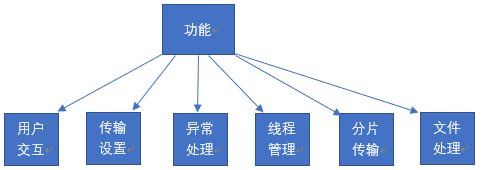
\includegraphics[width=11cm]{function.png}}
\caption{软件功能图}
\end{figure}
\subsection{用户交互模块}
如图3-4的软件功能图所示,展现的是断点续传软件的主要功能模块。其中,对于用户交互模块,需要实现的内容包括图形界面的设计,需要实现符合用户要求的图形界面接口,其中应包括主界面的设置,上传按钮的实现及对应的按钮监听的实现,下载按钮的实现以及对应的监听。对于文件上传部分,用户交互的要求还需要实现本地文件选择的界面窗口
当选择好要上传的文件后,还需实现文件传输的实时进度条的图形界面。
\par 对于文件下载部分,与文件上传略有区别,首先需要实现从服务器上选择已有完整文件的图形界面,在选择好待下载文件后同样需要显示文件实时传输进度的图形界面进度条。
\subsection{传输设置模块}
由于此断点续传软件需要遵守tus协议的基本传输要求,因此在软件功能中应该包含一块专门负责符合tus协议内容的文件传输设置的功能模块。此模块应该设置包含tus请求的基本格式,例如"HEAD","PATCH","OPTION"这样的请求字段,例如:如果要实现文件的新建上传功能,则应设置请求为"POST";如果要完成文件恢复上传的功能,则应设置请求为"HEAD",下载时与上传类似。除了设置tus请求,还要在与服务器的交互中附有tus协议标准的请求头部信息,例如:在文件的上传过程中,发送给服务器的请求里应包含Upload-Offset的字段以及对应的值,包含Upload-Metadata的字段以及对应值,Tus-Resumable的字段以及对应的值,以及客户端与服务端连接的timeout值设置。
\subsection{异常处理模块}
由于此软件设计使用JAVA语言实现,在此断点续传软件的运行过程中,以及代码的实现中,会出现不同种类的异常,例如:在操作文件时会出现IOException,NullPointException等异常,实现异常处理模块时,应针对可能出现某个特定异常的代码段中,利用JAVA语言的异常处理机制,添加对某个特定异常的捕获以及捕获异常后的程序段处理,这样使程序不会以为异常的出现,以及没有代码的处理,最终被JAVA虚拟机不断抛向上层函数并出现终端的报错信息。
\par 另外,对于可能出现的不符合tus协议标准的请求字段以及不在正常范围内的返回代码,也可以通过自定义异常的方式进行设置,不仅方便了对代码的管理,也对异常处理有了更标准的完善;针对软件的断点续传功能,本软件还设置了恢复选项异常,这个异常的意义在于:为文件的传输提供了可恢复选项,例如被定义为不可恢复传输的文件如果试图使用断点续传功能,则要求抛出这个恢复选项异常。
\subsection{线程管理模块}
此断点续传软件应为用户提供多线程的运行功能,如软件结构图3-1所示,用户通过图形界面来选择创建上传文件或下载文件的进程,每个被用户选择创建的新线程应拥有自己的线程id,以方便程序运行中报错及对线程操作的相关处理。由于断点续传软件所创建的线程的目的都是进行文件的传输,因此有很大的相似性,可以统一通过JAVA语言中的线程工厂对需要新创建的线程进行初始化,来减少代码的重复性,增加可读性。软件的主进程应拥有对各个子线程的控制权,包括线程的暂停,线程的恢复等。
\subsection{分片传输模块}
分片传输的功能模块是此断点续传软件的核心模块,他实现了文件的断点续传共能。如图3-3所示的分片传输原理图,通过对文件的分片来实现文件传输位置offset的等间隔记载,在恢复文件传输的工程中再使用offset的值,找到目标文件以及本地文件的传输位置,实现文件的可恢复传输功能。
\par 此外,文件分片的大小应有科学的设置:如果文件分片过大,则对于较小的文件,尤其是小于文件分片大小的文件,则失去了可恢复性传输的功能;如果文件分片过小,则程序运行时将在每个小文件分片传输完成后运行记录offset值得代码片段,而这个负责记录offset值得代码涉及到文件的写操作,因此,过大频率的写文件操作将给程序的运行带来负担,影响程序运行速度。所以,文件分片大小的设置应以符合用户的日常需求为准。
\subsection{文件处理模块}
此断点续传软件的功能实现过程中还将涉及到文件处理的内容,例如:在文件上传过程中,文件处理环节体现在本地文件的选取,并从客户端软件中提取此文件对上传所需要的信息,像文件长度、文件在本地系统中的绝对路径、文件名称等信息、以及若是恢复上传过程,在从服务器获取到文件上传位置offset的值之后,将在客户端程序中的文件对象上找到offset的位置,从这个暂停位置作为新一次上传的起始位置,获取到输入流当中,同时上传过程对服务器的文件也进行着操作,它体现在需要从客户端与服务端的连接中获取服务端目标文件的输出流,来进行新一次的文件写操作。由于tus协议本身在服务端并不提供服务端已有文件的查看接口,因此在完成一个文件的完整上传时,还要在本地做记录。
\par 在文件下载操作中,文件处理环节体现在本地文件的创建、从连接中获取服务端目标文件输入流的操作、从本地新建或已存在文件中提取输出流、在异常中断发生时或用户手动暂停下载时应有在本地记录文件传输位置offset值的处理。

\section{主要类的设计}
本传输软件的类设计符合软件需求的基本要求,主要包括显示客户端图形界面的界面类,负责文件传输及offset值记录的文件传输类,负责管理文件传输参数的客户端类等。
\subsection{TusClient类的设计}
\begin{figure}[h]
\subfigure{
\label{tusclient}
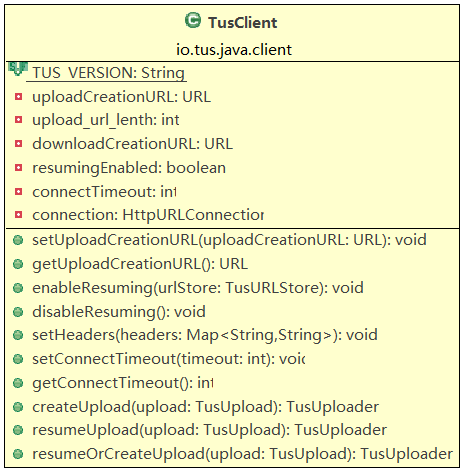
\includegraphics[width=9cm]{tusclient.png}}
\caption{TusClient类图}
\end{figure}
TusClient类主要负责通过接收的用户请求,在这里进行处理,完成uploader类doanloader类的初始化,为文件的传输功能做好准备。其中prepareConnection函数设置好了符合tus协议要求的请求格式,然后在创建上传函数,创建下载函数,回复上传函数,恢复函数对应不同的要求再单独添加的服务器请求条件。这样的设计减少了代码的重复,简化了结构,提高了可读性。
\par 其中的成员变量TUSVERSION记录了现在tus协议需要添加在请求中的tus版本号,因为在每次本地与服务器的交互中,请求头中都要添加这个内容,所以将他定义成了客户类中的一个成员变量,因为客户端程序中的从线程的打开只新建一个客户端类,并在这个客户端类的实例对象中进行对文件的各种操作,所以其他的文件传输设置都可以似乎用这个在外部的变量。uploadCreationURL变量记录了服务器ip地址及端口,resumingEnabled这个bool型变量记录了这个客户类及对应的任务线程是否允许开启恢复性传输。TusURLStore变量用来记录这个线程对应的本地文件与服务器文件的键值对,这个变量值存于客户端PC内存中。
\par 客户类的成员函数中包括对可恢复属性的开启、关闭以及获取属性的操作。resumeOrCreateUpload函数通过判断服务器是否有此本地文件对应的未完成上传的部分文件,来确定此次文件上传是新建上传还是恢复上传,后面的判断恢复或新建下载与此类似。与这个函数对应的两个函数分别时createUpload函数和resumeUpload函数,这两个函数分别完成对文件新建上传和文件恢复上传的信息初始化设置,并返回用于文件分片传输功能的uploader实例。setConnectionTimeout函数用于在此客户类实例外部设置连接超时时间,并且还包含获取超时时间接口。

\subsection{Window类的设计}
\begin{figure}[h]
\subfigure{
\label{window}
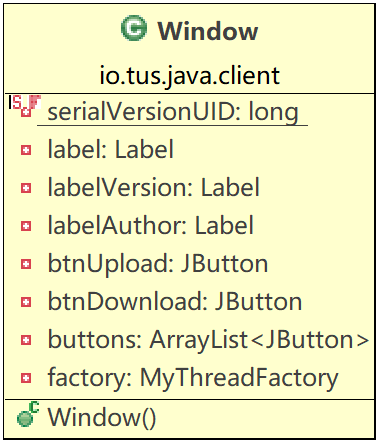
\includegraphics[width=5cm]{window.png}}
\caption{Window类图}
\end{figure}

\begin{figure}[h]
\subfigure{
\label{windowlistener}
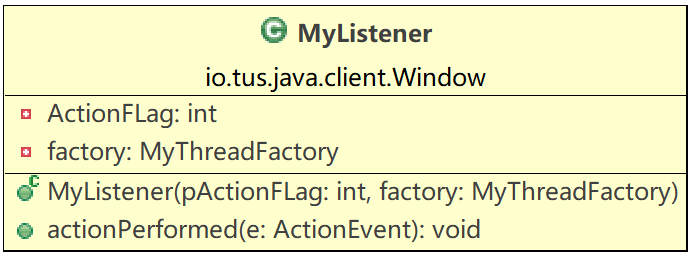
\includegraphics[width=9cm]{windowlistener.png}}
\caption{WindowListener类图}
\end{figure}
Window类的功能是负责用户图形界面的显示(如图3-6,3-7),其中Window初始化函数中设置了java中JFrame的窗口位置,窗口大小及相关字体的设置。MyListener类定义在Window类中,他的主要功能为监听Window窗口中的上传及下载按钮,并在这个监听类的功能函数中完成新建线程的处理。

\subsection{TusUpload类的设计}
TusUpload类用于封装选择的要上传的文件,并封装与文件有关的信息。在这个类中,size变量用于记录此待上传文件的大小,input变量由于设置文件的本地输入流。File类型的file变量用来记录这个文件的JAVA类对象,可以通过这个变量来获取待上传文件的文件名、文件大小、绝对路径等信息。metadata这个Map型的变量中,则记录了该文件的文件名,并在之后的连接服务器操作中附加在请求头部中。
\par 在成员函数中,带有File参数的TusUpload初始化函数通过待上传文件对象来初始化成员变量中的各个值,包括size,input,file,metadata,fingerprint等变量。其他函数均为设置或获取upload对象中封装的待上传文件信息的操作,因为这个类的设计思路就是在线程运行中初步封装待上传的文件信息,然后通过客户类中的功能函数来最终确定文件分片传输所需要的uploader对象,再通过调用uploader中的函数来完成分片上传的软件功能。

\subsection{JProcessBar类的设计}
\begin{figure}[h]
\subfigure{
\label{jprocessbar}
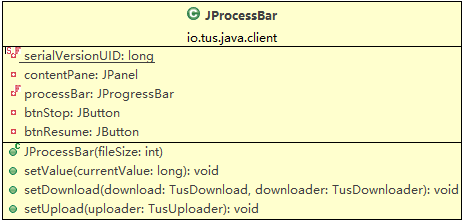
\includegraphics[width=9cm]{jprocessbar.png}}
\caption{JProcessBar类图}
\end{figure}
JProcessBar类主要负责将实时的offset值用进度条的图形方式显示出来。进度条窗口应对应着一个已创建的线程,为这个线程所运行的文件上传或文件下载过程提供实时的进度条图形界面显示。此外,这个进度条类还应包含着用于控制这个线程文件传输过程的暂停传输和恢复传输按钮。
\par 在此类的成员变量中,应包含用于显示此进度条的JAVA窗口容器JPanel对象。btnStop变量和btnResumme变量均为JButton类型的对象,用于表示并实现暂停文件传输和恢复文件传输的按钮,在这个进度条类中还分别对应暂停传输和恢复传输按钮编写监听类,并在对应的监听类中实现当前线程的结束以及建立新的线程以实现恢复文件传输的操作。
\par 在此类的成员函数中,带有整型变量fileSize的参数的初始化函数通过传入的目标文件的大小来确定构成进度条中的总数据大小。而于此对应,需要override的函数setValue将在每次分块传输完成时将此时此刻的文件传输进度offset的值传入并调用此函数,以此来实现进度条对文件传输位置的实时图形显示。

\subsection{TusUploadRun类的设计}
\begin{figure}[h]
\subfigure{
\label{tusuploadrun}
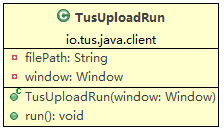
\includegraphics[width=5cm]{tusuploadrun.png}}
\caption{TusUploadRun类图}
\end{figure}
这个类负责为线程提供用于本软件文件传输功能的接口,TusUploadRun类与TusDownloadRun类基本相似。
\par 在这个类中的功能函数TusUploadRun中,将完成一个新建线程中从TusClient类的初始化,TusUpload类的对文件的封装过程,进度条类的初始化,到调用客户类的功能函数,最终生成uploader对象或downloader对象的分片传输所需的内容。在生成了传输容器对象后,还将通过循环和对容器对象分片传输函数的调用来实现文件的分片传输功能并在每次分片传输完成时进行配置文件的写操作和进度条的更新操作。这个类功能函数的实现将在第四章中呈现。

\subsection{主要类间的关系}
\par 如图3-10,展示了Window类,TusUploadRun类间的调用关系。window中的监听按钮收到信号时,将新建上传线程,而TusUploadRun则是线程运行的接口。
\par 在Window类所创建的断点续传软件主窗口中,分别包含着下载和上传按钮,用户同过这两个按钮的点击来出发监听类的运行,监听类通过判断用户操作来通过MyThreadFactory线程工厂类创建新的线程,同时确定用户所需的上传或下载操作。如果是上传操作,则对应将TusUploadRun接口传入到线程工厂中,从而在这个新建线程里运行的就是接口里定义的文件上传的一系列操作,正如上一节所描述的TusUploadRun类的介绍那样;如果是下载操作,同理,监听类将把文件下载运行接口传入线程工厂中,从而运行接口里定义的文件下载的一系列操作。在图3-10中由于空间大小,没有画出TusDownRun类与他们间的关系,但此类应与TusUploadRun类的关系相似。
\begin{figure}[h]
\subfigure{
\label{4class}
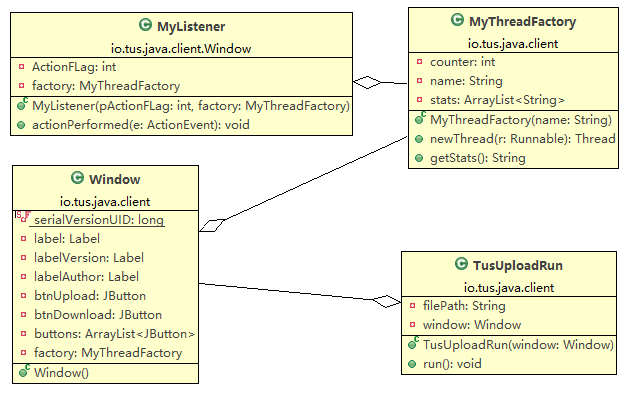
\includegraphics[width=12cm]{4class.png}}
\caption{Window类,TusUploadRun类的关系}
\end{figure}
\par 如图3-11所示,展示了TusClient类与TusUploader类、TusDownloader类的关系。在TusClient类中,通过对象的成员函数例如开始上传函数、恢复上传函数、开始下载函数、恢复下载函数。在上传过程中,程序将通过服务器上是否有相同文件来决定是否新建上传或恢复上传,并返回一个TusUploader类型的对象,在这个对象中包含着上传此文件所需的信息;在下载过程中,程序将通过本地是否有与选择文件相同的文件来决定是否新建下载或恢复下载,并返回一个Tus下载容器类型的对象,这个对象的私有成员变量中包含着下载此文件所需的所有信息。所以传输文件所需的内容,包含服务器url、目标文件长度、文件传输进度offset的值、文件存储位置等,这些都分别包含在了两个上传、下载容器中,这两个容器同时拥有着对文件传输起着至关重要作用的分片传输功能函数,而客户端类的作用就是对这两个容器类进行配置和初始化,以此来完成对传输的控制。
\begin{figure}[h]
\subfigure{
\label{3class}
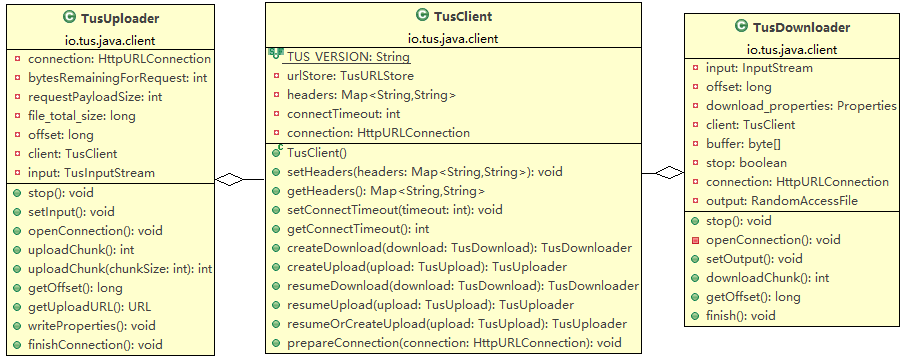
\includegraphics[width=12cm]{3class.png}}
\caption{客户类和上传下载类的联系}
\end{figure}

\section{软件流程设计}
此软件为用户创建了图形界面,在界面中可自行选择上传文件或下载文件的操作。
\par 当使用上传功能时,程序会通过java提供的文件选择工具选择上传文件,并通过与服务器的连接并获取此文件在服务器上是否有部分或完整的镜像,若只有部分上传则会通过服务器返回的response回复提供给此客户端程序上传的进度信息,即offset字段。
\par 当使用下载功能时,程序会通过本地记录的配置文件获取此时服务器上已有的完整文件名,以供下载选择,此时程序会提供用户选择本地文件来开始或继续下载此文件,程序通过配置文件获取本地未完成下载文件的offset值,并继续下载。

\subsection{UML流程图}
统一建模语言(英语:Unified Modeling Language,缩写 UML)是非专利的第三代建模和规约语言。UML是一种开放的方法,用于说明、可视化、构建和编写一个正在开发的、面向对象的、软件密集系统的制品的开放方法。UML展现了一系列最佳工程实践,这些最佳实践在对大规模,复杂系统进行建模方面,特别是在软件架构层次已经被验证有效。
\begin{figure}[h]
\subfigure{
\label{liucheng}
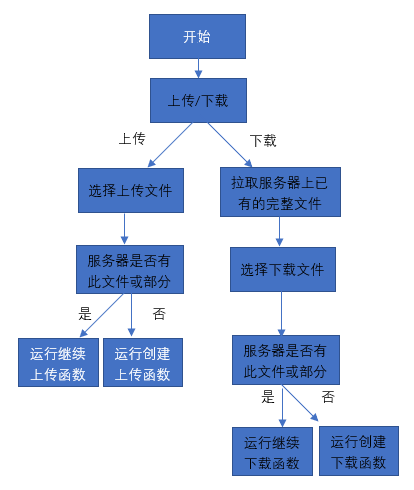
\includegraphics[width=10cm]{liucheng.png}}
\caption{断点续传软件流程图}
\end{figure}
\par 如图3-12所示的断点续传软件流程图,程序开始运行,将首先显示出Window类展现的主界面,上面要包含着上传文件和下载文件两个按钮。通过这两个按钮的监听类,程序将确定用户的选择,并进行分别的处理。就如图3-10所示的类图关系中的调用一样:如果用户选择的是上传操作,程序在运行TusUploadRun接口定义的线程时,就等于运行了如图3-12左边上传流程,其中服务器是否有此文件或部分的内容,包含在了初始化TusClient类以及调用这个客户类中的判别函数来实现,确定了这个之后,就是通过调用两个传输容器uploader以及downloader类中的分片传输函数来实现文件的分片传输过程。
\par 如果用户选择的是下载操作,则程序将运行图3-12右边下载部分的流程。程序首先将为用户用图形界面的方式提供服务器上已存在的完整文件以供用户选择,选择好待下载文件后,程序同样初始化TusClient类,并调用判别创建下载或恢复下载函数来确定接下来需要进行的操作,同时将文件信息封装在TusDownloader类的实例中,后面的代码与上传函数一样,实现文件的分片传输。以上流程和程序代码的实现都包含于TusDownloadRun接口的运行函数中,它定义了这个新建线程的操作。

\section{本章小结}
本章主要介绍了断点续传软件的需求分析,运行原理,和java代码的分类设计,分别对主要类进行了关键函数说明。可以看到,软件在遵循tus协议文件传输规则的同时,通过分片传输机制实现了断点续传功能,这也是此次毕业设计的核心任务。

\chapter{软件的实现}
\section{程序主要类的介绍}
此程序的主要文件传输功能函数封装在了tusuploader和tusdownloader两个类中,其他类完成其他基本参数传递,配置文件以及图形界面的需求。

\subsection{Window类}
客户端界面的基本设置:
\begin{lstlisting}[title=主界面的设置]
	public Window() {
		super("tus断点续传客户端");
		this.setBounds(0, 0, 500, 260);
		this.setVisible(true);
		this.setDefaultCloseOperation(JFrame.EXIT_ON_CLOSE);
		this.getContentPane().setLayout(null);
		this.setLocationRelativeTo(null);
		buttons.add(btnUpload);
		buttons.add(btnDownload);
		label.setBounds(100, 10, 260, 30);
		label.setText("tus java client");
		label.setFont(new java.awt.Font("MS Tang", Font.BOLD, 20));
		this.getContentPane().add(label);
		labelVersion.setBounds(360, 18, 50, 20);
		labelVersion.setText("v1.0");
		labelVersion.setFont(new java.awt.Font("MS Tang", Font.BOLD, 15));
		this.getContentPane().add(labelVersion);
		labelAuthor.setBounds(350, 30, 150, 30);
		labelAuthor.setText("2018.4    by Tzz");
		labelAuthor.setFont(new java.awt.Font("MS Tang", Font.ITALIC, 10));
		this.getContentPane().add(labelAuthor);
		btnUpload.setBounds(50, 60, 180, 30);
		this.getContentPane().add(btnUpload);
		btnDownload.setBounds(50, 100, 180, 30);
		this.getContentPane().add(btnDownload);
		//设置监听
		for (int i = 0; i < buttons.size(); i++)
		{
			buttons.get(i).addActionListener(new MyListener(i, factory));
		}
	}
\end{lstlisting}
\par Window类继承了JFrame类,这个公共的Window类构造函数完成了基本的界面设置,8-9行将上传和下载按钮添加到了ArrayList<JButton> buttons中,便于管理,并在23,25行将两个按钮添加到了window容器中。用JButton类中的addActionListener函数为两个按钮添加监听。监听类如下所示:
\begin{lstlisting}[title=监听的编写]
private class MyListener implements ActionListener {
		private int ActionFLag = -1;
		private MyThreadFactory factory = new MyThreadFactory("MyThreadFactory");
		public MyListener(int pActionFLag, MyThreadFactory factory)
		{
			this.ActionFLag = pActionFLag;
			this.factory = factory;
		}
		
		@Override
		public void actionPerformed(ActionEvent e) {  //上传
			switch (this.ActionFLag) {
			case 0:  //上传
				TusUploadRun run1 = new TusUploadRun(Window.this);
				Thread thread1;
				thread1 = factory.newThread(run1);
				thread1.start();
				break;
				
			case 1:  //下载
				TusDownloadRun run2 = new TusDownloadRun();
				Thread thread2;
				thread2 = factory.newThread(run2);
				thread2.start();
				break;
				
			default:
				break;
			}
		}
	}
\end{lstlisting}
\par 通过MyListener类中的整形变量ActionFlag来确定应响应上传操作还是下载操作,并在前面的Window类构造函数中进行对应的初始化。上传和下载模块分别初始化了TusUploadRun和TusDownloadRun两个继承了Runable类的对象,并通过线程工厂分别创建了负责文件传输的线程。

\subsection{MyThreadFactory类}
MyTreadFactory构造函数:
\begin{lstlisting}[title=MyThreadFactory的构造函数]
public MyThreadFactory(String name) {
		counter = 0;
		this.name = name;	
		stats = new ArrayList<String>();
	}
\end{lstlisting}
\par 构造函数中初始化了计数器counter,用于记录线程工厂创建的线程数量,工厂类名字,和用于记录每个创建出的线程状态的ArrayList。
\begin{lstlisting}[title=MyThreadFactory的创建新线程函数]
@Override
public Thread newThread(Runnable r) {
	Thread t = new Thread(r, name + "-Thread_" + counter);
	counter++;
	stats.add(String.format("created thread %d with name %s on %s\n", t.getId(), t.getName(), new Date()));	
	return t;
	}
\end{lstlisting}
\par 这个Override函数为线程工厂中最重要的功能函数,他接受一个Runnable对象参数,并在函数中通过传递Runnable接口的方式创建新线程,此线程的start()方法运行的便是Runnable接口中定义的过程。这个线程工厂基本完成了软件设计阶段所需要的需求。

\subsection{TusUploadRun类}
TusUploadRun类继承了java提供的Runnable类,这个类可以通过接口传给新建线程,使线程完成此类里完成的功能。
\begin{lstlisting}[title=TusUploadRun类中的线程运行函数]
@Override
public void run() {
	JFileChooser chooser = new JFileChooser();
	chooser.setFileSelectionMode(JFileChooser.FILES_AND_DIRECTORIES);
	int r = chooser.showOpenDialog(window);
	if (r == JFileChooser.APPROVE_OPTION) {
		// 设置文件路径
		filePath = chooser.getSelectedFile().getPath();
	}
	try {
		System.setProperty("http.strictPostRedirect", "true");
		final TusClient client = new TusClient();
		client.setUploadCreationURL(new URL("http://localhost:1081/files"));
		File file = new File(filePath);
		final TusUpload upload = new TusUpload(file);
		TusURLMemoryStore tus_url_store = new TusURLMemoryStore();
		client.enableResuming(tus_url_store);
		System.out.println("Starting upload...");
		TusUploader uploader = client.resumeOrCreateUpload(upload);
		uploader.setChunkSize(1024);
		// 设置进度条
		 JProcessBar process_bar = new JProcessBar((int)upload.getSize());
		 process_bar.setUpload(uploader);
		do {
			process_bar.setValue(uploader.getOffset());
		} while (uploader.uploadChunk() > -1);
		uploader.finishConnection();;
		if (uploader.getOffset() == uploader.getFileTotalSize()) {
			System.out.println("Upload finished.");
			System.out.format("Upload available at: %s", uploader.getUploadURL().toString());
			uploader.writeProperties();
		}
	} catch (Exception e1) {
		e1.printStackTrace();
	}
}
\end{lstlisting}
\par 此类中包含的run函数即为线程运行的代码,其中包括弹出文件选择窗口,将选中文件传递给设置函数。其中run函数的第13行规定了服务端的ip地址和端口及文件存储路径,由于没有进行过远程测试,因此这个服务器地址没有给出用户接口,而仅仅在这里进行了规定。第19行调用的函数为TusClient类中的关键函数,此函数用来运行恢复上传或新建上传的准备工作,包括恢复上传中的从服务器获取offset值以及新建上传中写配置文件等。client对象调用的这个函数返回了一个TusUploader类的对象,这个对象用来在下面的循环按块上传中调用传输函数。第22行中的JProcessBar类为自定义类,这个类创建了一个新的窗口,用来实时显示文件传输的进度,并在第25行这个while循环中每次更新进度条的显示值。第26行为循环上传的判断条件,同时也是进行数据传输的函数。
\par 由于在新弹出的任务窗口中提供了以中断与服务器连接的方式中断传输,并因此调出这个while循环,所以要在第28对是否完成传输进行判断。

\subsection{TusUpload类}
TusUpload类主要完成文件上传的输入流设置,以及base64的文件名加密操作。
\begin{lstlisting}[title=TusUpload类构造函数]
public TusUpload(@NotNull File file) throws FileNotFoundException {
        size = file.length();
        this.file = file;
        setInputStream(new FileInputStream(file));
        fingerprint = String.format("%s-%d", file.getAbsolutePath(), size);
        metadata = new HashMap<String, String>();
        metadata.put("filename", file.getName());
        local_file_path = file.getAbsolutePath();
    }
\end{lstlisting}
\par 在这个构造函数中,主要初始化了输入流,这里的输入流为自定义的TusInputStream类,这个类对普通的文件输入流进行了封装和简单的添加功能。
\begin{lstlisting}[title=base64加密函数]
static String base64Encode(byte[] in)       {
        StringBuilder out = new StringBuilder((in.length * 4) / 3);
        String codes = "ABCDEFGHIJKLMNOPQRSTUVWXYZabcdefghijklmnopqrstuvwxyz0123456789+/=";
        int b;
        for (int i = 0; i < in.length; i += 3)  {
            b = (in[i] & 0xFC) >> 2;
            out.append(codes.charAt(b));
            b = (in[i] & 0x03) << 4;
            if (i + 1 < in.length)      {
                b |= (in[i + 1] & 0xF0) >> 4;
                out.append(codes.charAt(b));
                b = (in[i + 1] & 0x0F) << 2;
                if (i + 2 < in.length)  {
                    b |= (in[i + 2] & 0xC0) >> 6;
                    out.append(codes.charAt(b));
                    b = in[i + 2] & 0x3F;
                    out.append(codes.charAt(b));
                } else  {
                    out.append(codes.charAt(b));
                    out.append('=');
                }
            } else      {
                out.append(codes.charAt(b));
                out.append("==");
            }
        }
        return out.toString();
    }
\end{lstlisting}
虽然jdk中java.util.Base64已经包含类base64的加密方法,但这里还是用java代码简单实现了base64的功能。

\subsection{TusUploader类}
Uploader类中封装了上传文件所需要的所有信息,只要传递这个类,就可以灵活的其他位置进行传输。其中最重要的成员函数为uploadChunk()函数。
\begin{lstlisting}[title=上传函数]
public int uploadChunk() throws IOException, ProtocolException {
        openConnection();
        if (stop) {
    		stop = false;
    		return -1;
    	}
        int bytesToRead = 1024;
        int bytesRead = input.read(buffer, bytesToRead);
        if(bytesRead == -1) {
        	return -1;
        }
        output.write(buffer, 0, bytesRead);
        output.flush();
        offset += bytesRead;
        bytesRemainingForRequest -= bytesRead;
        if (input == null) return -1;
        return bytesRead;
    }
\end{lstlisting}
\par 当boolean型变量stop的值为true时,将退出这个块传输循环。传输过程为,在输入流中读取设置的块大小1KB的数据,读入buffer缓冲区中,然后再从buffer传入输出流中。
\begin{lstlisting}[title=从连接中获取输出流]
output = connection.getOutputStream();
\end{lstlisting}
这里,上传的输出流为从与服务器的连接类中获取的。下载过程中的TusDownload类和TusDownloader类与上传类似,最大的区别在于下载的输入流来自与服务器连接中,而输出流为本地的用户创建的文件。
\begin{lstlisting}[title=tus协议中的新建上传POST]
HttpURLConnection connection = (HttpURLConnection) uploadCreationURL.openConnection();
connection.setRequestMethod("POST");
\end{lstlisting}
\par 上传文件的请求也遵循了tus协议的内容,设置了POST方法。而下载时则是GET。

\subsection{关于配置文件}
程序一共管理了三个配置文件:
\par 1.config.properties文件:记录了本地文件绝对路径与服务器对应传输文件的键值对,便于在恢复上传时查询此文件,找到服务器对应的未完成文件。
\par 2.serverfile.properties文件:每当程序检查完成一个文件的完整上传时,会记录该文件在服务器上的绝对路径。
\begin{lstlisting}[title=记录服务器中存在的完整文件]
Properties properties = new Properties();
properties.load(new FileInputStream("F:\\Workspace_for_jee\\tus-java-client-master\\server_file.properties"));
properties.setProperty(uploadURL.toString(), "ture");
properties.store(new FileOutputStream("F:\\Workspace_for_jee\\tus-java-client-master\\server_file.properties"), "上传完成的文件");
\end{lstlisting}
\par downloadoffset.properties文件:用于在下载文件时在本地保存文件下载位置offset的值,文件中保存的是本地保存文件的绝对路径和此文件offset值的键值对。因为在程序运行时,若每次块下载循环完成就写一次offset值,这样的方式严重影响了下载速度,所以设计为每下载10MB的文件大小时再记录一次offset,如果通过展厅按钮方式暂停下载时就即刻记录offset。

\section{本章小结}
本章节详细介绍了基于tus协议的断点续传客户端软件的核心类的功能及代码实现,可以看出代码的编写基本符合了软件需求的设定,完成了tus协议规定的报文标准、通过分块传输以实现断点续传功能、以及多线程管理的实现。

\chapter{软件的测试}
\section{软件测试的概念}
软件测试(英语:software testing),描述一种用来促进鉴定软件的正确性、完整性、安全性和品质的过程。据此,您可能会想,软件测试永远不可能完整的确立任意电脑软件的正确性。然而,在可计算理论(计算机科学的一个支派)一个简单的数学证明推断出下列结果:不可能完全解决所谓“死机”,指任意计算机程序是否会进入死循环,或者罢工并产生输出问题。换句话说,软件测试是一种实际输出与预期输出间的审核或者比较过程。
\par 软件测试的经典定义是:在规定的条件下对程序进行操作,以发现程序错误,衡量软件品质,并对其是否能满足设计要求进行评估的过程。

\section{本软件的测试}
\subsection{软件测试用例}
测试用例(Test Case)是为某个特殊目标而编制的一组测试输入、执行条件以及预期结果,以便测试某个程序路径或核实是否满足某个特定需求。
\subsection{软件测试环境}
本软件的测试环境为windows10,64位系统,IDE使用的是eclipse java mars,测试工具为JUnit,JUnit是一个Java语言的单元测试框架。它由肯特·贝克和埃里希·伽玛(Erich Gamma)建立,逐渐成为源于Kent Beck的sUnit的xUnit家族中为最成功的一个。 JUnit有它自己的JUnit扩展生态圈。
\subsection{软件的详细测试}
此断点续传软件中,对一些重点类进行了测试函数的编写,内容如下。
\subsubsection{TestTusClient测试类}
\begin{lstlisting}[title=testTusClientURL测试函数]
    @Test
    public void testTusClientURL() throws MalformedURLException {
        TusClient client = new TusClient();
        client.setUploadCreationURL(creationUrl);
        assertEquals(client.getUploadCreationURL(), creationUrl);
    }
\end{lstlisting}
\par testTusClientURL函数用于检查client对象中的上传地址是否正确。

\begin{lstlisting}[title=testSetUploadCreationURL测试函数]
    @Test
    public void testSetUploadCreationURL() throws MalformedURLException {
        TusClient client = new TusClient();
        client.setUploadCreationURL(new URL("http://master.tus.io"));
        assertEquals(client.getUploadCreationURL(), new URL("http://master.tus.io"));
    }
\end{lstlisting}
\par testSetUploadCreationURL函数用于测试TusClient类中的setUploadCreationURL函数的可用性。

\begin{lstlisting}[title=testEnableResuming测试函数]
    @Test
    public void testEnableResuming() {
        TusClient client = new TusClient();
        assertEquals(client.resumingEnabled(), false);

        TusURLStore store = new TusURLMemoryStore();
        client.enableResuming(store);
        assertEquals(client.resumingEnabled(), true);

        client.disableResuming();
        assertEquals(client.resumingEnabled(), false);
    }
\end{lstlisting}
\par testEnableResuming函数用于测试TusClient类中的EnableResuming函数。当初始化TusClient类的对象时,对象中的可恢复属性初试为false,当用TusURLStore类进行服务器文件地址URL存储时,将自动将client对象中的可恢复上传属性设置为true。当调用disableResuming函数时,可恢复属性又变回false。

\begin{lstlisting}[title=testPrepareConnection测试函数]
    @Test
    public void testPrepareConnection() throws IOException {
        HttpURLConnection connection = (HttpURLConnection) mockServerURL.openConnection();
        TusClient client = new TusClient();
        client.prepareConnection(connection);

        assertEquals(connection.getRequestProperty("Tus-Resumable"), TusClient.TUS_VERSION);
    }
\end{lstlisting}
\par testPrepareConnection函数用于测试TusClient类中的tPrepareConnection函数是否可用。此测试使用mockServerURL地址打开连接,初始化客户端类后调用prepareConnection函数,并对照从连接中获取的tus版本号与本地新建的客户端类tus版本号是否一致。

\begin{lstlisting}[title=testSetHeaders测试函数]
    @Test
    public void testSetHeaders() throws IOException {
        HttpURLConnection connection = (HttpURLConnection) mockServerURL.openConnection();
        TusClient client = new TusClient();

        Map<String, String> headers = new HashMap<String, String>();
        headers.put("Greeting", "Hello");
        headers.put("Important", "yes");
        headers.put("Tus-Resumable", "evil");

        assertNull(client.getHeaders());
        client.setHeaders(headers);
        assertEquals(headers, client.getHeaders());

        client.prepareConnection(connection);

        assertEquals(connection.getRequestProperty("Greeting"), "Hello");
        assertEquals(connection.getRequestProperty("Important"), "yes");
    }
\end{lstlisting}
\par testSetHeaders函数用于测试TusClient类中的SetHeaders函数的功能。在代码的7,8,9行中分别对headers进行内容填充,然后分别从本地初始化的客户端类和建立的与服务器的连接中获取键值对,查看是否与预期值对应。
\par 用JUnit运行的TestTusClient类测试结果如图5-1所示:
\begin{figure}[h]
\subfigure{
\label{TestTusClient}
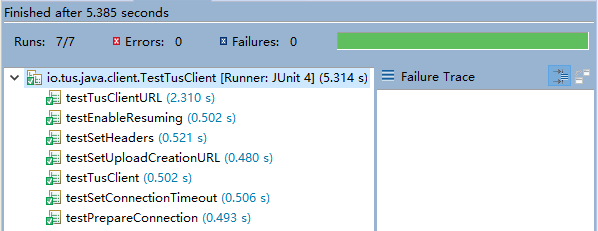
\includegraphics[width=12cm]{testtusclient.png}}
\caption{TestTusClient测试类的运行例子}
\end{figure}

\subsubsection{TestTusUpload测试类}
\begin{lstlisting}[title=testTusUploadFile测试函数]
    @Test
    public void testTusUploadFile() throws IOException {
        String content = "hello world";

        File file = File.createTempFile("tus-upload-test", ".tmp");
        OutputStream output = new FileOutputStream(file);
        output.write(content.getBytes());
        output.close();

        TusUpload upload = new TusUpload(file);

        Map<String, String> metadata = new LinkedHashMap<String, String>();
        metadata.put("foo", "hello");
        metadata.put("bar", "world");
        metadata.putAll(upload.getMetadata());

        assertEquals(metadata.get("filename"), file.getName());

        upload.setMetadata(metadata);
        assertEquals(upload.getMetadata(), metadata);
        assertEquals(
                upload.getEncodedMetadata(),
                "foo aGVsbG8=,bar d29ybGQ=,filename " + TusUpload.base64Encode(file.getName().getBytes()));

        assertEquals(upload.getSize(), content.length());
        assertNotSame(upload.getFingerprint(), "");
        byte[] readContent = new byte[content.length()];
        assertEquals(upload.getInputStream().read(readContent), content.length());
        assertEquals(new String(readContent), content);
	}
\end{lstlisting}
\par TestTusUpload测试类和testTusUploadFile测试函数用于测试upload类中的管理文件信息的函数的正确性。测试函数首先在本地创建一个用于测试的临时文件tus-upload-test.tmp,将hello world写如此文件中,然后通过upload对象的getMetadata函数提取初始化upload时设置的信息,与本地新建的文件信息对比。
\par 测试类的运行结果如图5-2所示:
\begin{figure}[h]
\subfigure{
\label{TestTusUpload}
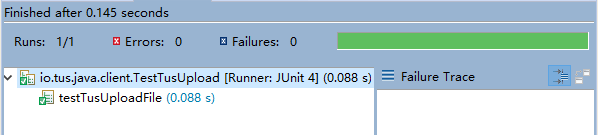
\includegraphics[width=12cm]{testtusupload.png}}
\caption{TestTusUpload测试类的运行例子}
\end{figure}

\section{软件的使用}
如图5-3所示,展示的是客户端软件在选择本地待上传文件时的图形界面。
\begin{figure}[h]
\subfigure{
\label{upload}
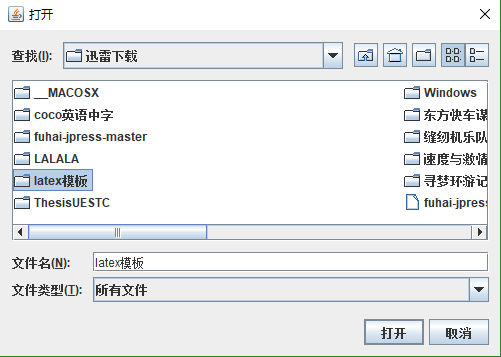
\includegraphics[width=12cm]{upload.png}}
\caption{断点续传软件上传功能}
\end{figure}
\par 如图5-4所示,展示的是软件从服务器获取已存在的完整文件的示意图,在这个下拉菜单中将显示所有已有的完整文件,当用户点击确定后将会出现图5-3所示类似的创建本地接收文件或选择本地已下载部分的文件,来完成文件的创建下载或恢复下载。
\begin{figure}[h]
\subfigure{
\label{download}
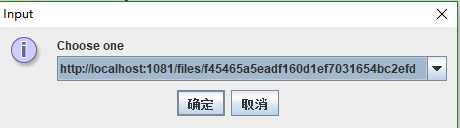
\includegraphics[width=12cm]{download.png}}
\caption{从服务器选择文件}
\end{figure}
\par 如图5-5所示,展示的是断点续传软件多线程完成用户任务的示意图,可以让用户分别操作不同线程控制的文件传输过程,而其他线程的任务运行不受影响。虽然程序没有设定最大允许的活动线程数量,但是由于网络等硬件条件的限制,当多个线程同时进行文件传输时,传输速度将受到较大影响。得出这个结论的依据是当启用多个线程时,文件进度条进度明显变慢,但将其他传输线程暂停支流单个线程时,传输速度将会恢复到单独运行的水平。
\begin{figure}[h]
\subfigure{
\label{upanddown}
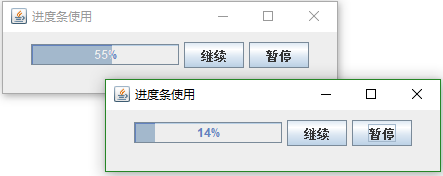
\includegraphics[width=12cm]{upanddown.png}}
\caption{上传和下载并行运行}
\end{figure}
\par 由于本软件采用的是分片传输原理,因此当特殊故障发生使得程序崩溃或停止运行时,不会影响到文件传输位置offset的记录。


\section{本章小结}
本章通过运行tusd服务器与本软件进行程序黑箱测试,包括文件的上传、下载以及多线程运行。并通过测试类函数的编写,利用JUnit工具完成了部分类功能函数的数据测试,及结果展示。

\chapter{全文总结与展望}

\section{全文总结}
本文以tus协议为基础,介绍了tus协议的基本内容,然后对软件的需求分析,模块设计进行了详细说明,最后是软件的运行测试。tus断点续传软件以http协议为基础,遵循tus协议的规定标准,并采用分块循环传输的方式来记录文件传输过程中的传输位置,用配置文件的方式记录本地offset以完成断点续传的功能。


\section{后续工作展望}
在tus协议中,还有很多附加的传输功能,能够使服务器与客户端间更加便捷的通信。按照tus协议标准,在服务器端存储的文件名称是软件自行定义的,所以从服务器拉取文件时文件名称不容易被用户接受,可以添加用户自定义文件名称,与tus规定的文件名称一一对应。
\par 由于此软件在进行文件传输时的运行传输函数和进度条窗口以及包含的暂停恢复按钮是在同一个线程中定义的,所以不能通过单纯的在此线程外部停止和恢复线程运行,这是本软件多线程管理中不方便的地方,但是可以通过把文件传输函数和文件传输过程的进度条显示分到两个线程的方式来改进,这就可以通过传参的方式实时更新进图条的值,并且可以在运行函数的线程外部轻松的调用JAVA线程机制,来暂停和恢复线程的运行。同时使用java多线程时可以添加java线程池的使用,从而更加方便的对正在运行的线程进行管理。

\thesisacknowledgement
在进行毕业设计期间,首先衷心感谢我的导师丘志杰老师对我的认真督促和帮助。在项目的实现过程中也遇到很多困难,同时也感谢给予我帮助的同学。


\thesisloadbibliography{reference}

%
% Uncomment following codes to load bibliography database with native
% \bibliography command.
%
% \nocite{*}
% \bibliographystyle{thesis-uestc}
% \bibliography{reference}
%

%添加附录页
%\thesisappendix

\thesisloadachievement{publications}


\thesistranslationoriginal
\section{A protocol for resumable file uploads}
With mobile devices becoming the dominant source of user generated media files, reliable file uploading through unreliable mobile networks has become an important issue for anybody interested in content acquisition.

Reliability here means the ability to detect network errors, and resuming an upload without having to start from the beginning. In many scenarios this can mean the difference between a file reaching your application, or the user giving up in frustration.

Ideally, this should be a trivial feature to add. In reality however, there is quite a lack of solutions in this space. Sure, there are a few JavaScript libraries that claim to support resumable uploading, but in reality you will end up spending a lot of time coming up with your own API for it, or implementing a poorly specified one specific to a library. This is incredibly frustrating, especially if you are planning to support this feature on multiple platforms such as HTML5, iOS and Android.

Now, if you’re a big company like Google, you may sit down and create such a protocol for your needs. And in fact, Google has been working on a such a protocol since 2010, for the now defunct Google Gears. The latest incarnation of this are two incompatible protocols for Google Drive and YouTube. But unfortunately both of these protocols rely on a non-standard http status code (308 Resume Incomplete), and are far from being generic enough for general adoption.

This means that smaller companies are currently doomed to invent, implement and maintain their own incompatible protocols and solutions for something that should be a trivial component of a modern application.

We find this unacceptable, so the tus project is a community project that was born in order to level the playing field and make resumable file uploading easy for anybody to implement.

As time progresses, we share ever larger media files from our phones and desktops. More than often, however, complications arise during this process. Whether it is through servers misbehaving or mobile users switching to a WiFi connection, the outcome is the same: ‘upload interrupted’.

This is by itself a negative user experience, but it becomes even worse when it happens in the middle of a 2GB upload on a slow connection. And of course, the longer an upload takes, the more exposed it is to poor connections. A failed upload will then have to be retried from the start, if the user even bothers with it at all.

With media files growing larger and networks remaining fragile, it is clear that we need a better solution to handle uploading.

\begin{figure}[h]
\subfigure{
\label{tus.io}
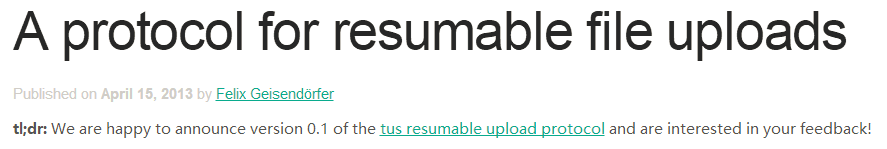
\includegraphics[width=15cm]{tusio.png}}
\caption{blog on tus.io}
\end{figure}

\thesistranslationchinese
\section{用于可恢复文件上传的协议}
随着移动设备成为用户生成媒体文件的主要来源,通过不可靠的移动网络进行可靠的文件上传已成为任何对内容获取感兴趣的人的重要问题。

这里的可靠性意味着能够检测网络中出现的错误,并且无需从头开始即可恢复上传的特性。在许多情况下,这可能意味着文件到达您的应用程序或用户放弃挫败之间的差异。

理想情况下,这应该是一个微不足道的功能。但事实上,在这个领域还缺乏解决方案。当然,有一些JavaScript库声称支持可恢复上传,但事实上,你最终会花费大量时间为自己的API提供自己的API,或者实现一个针对库的错误指定的API。这非常令人沮丧,特别是如果您打算在多个平台(如HTML5,iOS和Android)上支持此功能。

现在,如果你是像Google这样的大公司,你可以坐下来为你的需求创建一个这样的协议。事实上,谷歌自2010年以来一直在制定这样的协议,目前已停止使用Google Gears。这是Google Drive和YouTube的两个不兼容的协议。但不幸的是,这些协议都依赖于一个非标准的http状态代码(308 Resume Incomplete),并且远远不够通用。

这意味着小公司现在注定要发明,实施和维护他们自己的不兼容的协议和解决方案,以应对现代应用中微不足道的组件。

我们发现这是不可接受的,所以tus项目是一个社区项目,它的诞生是为了平衡竞争环境,并使任何人都可以轻松实现可恢复的文件上传。

随着时间的推移,我们会从手机和台式机共享更大的媒体文件。 然而,在这个过程中往往会出现复杂情况。 无论是通过服务器行为异常还是移动用户切换到WiFi连接,结果都是一样的:“上传中断”。

这本身就是一种负面的用户体验,但当它发生在缓慢连接的2GB上传中间时,它变得更糟。 当然,上传时间越长,连接不良就越暴露。 如果用户甚至无法使用,上传失败将不得不从一开始就重新尝试。

随着媒体文件越来越大,网络保持脆弱,很显然我们需要更好的解决方案来处理上传。

\end{document}
